\subsection{Explication de la mémoire}
Pour comprendre les résultats précédents nous devons étudier brièvement l'architecture des ordinateurs.
%
Les performances d'un ordinateur dépendent essentiellement de deux choses : le processeur et la mémoire.
%
Quand un programme souhaite lire une donnée en mémoire, il subit une pénalité mémoire.
%
Cette pénalité est la somme de deux contraintes :
\begin{itemize}
        \item la latence : la différence de temps entre la demande d'accès à la mémoire et la réception du premier octet;
        \item la bande passante : le nombre maximum d'octet par seconde que le bus peut envoyer/recevoir
\end{itemize}
%
De nos jours, les ordinateurs ont différents types de mémoires.
%
Il y a la mémoire cache, très proche des unités de calcul, elle a une faible latence (quelques cycles) mais sa taille est limité à quelques Mo.
%
Ensuite, il y a la mémoire RAM avec une latence de quelques centaines de cycles mais avec une taille de plusieurs Go.
%
Si nous regardons la structure mémoire de deux bancs NUMA de la figure~\ref{fig:numa_architecture}, on s'aperçoit que la distance physique des coeurs de calcul et de la mémoire est liée à la latence des accès mémoires.
%
Pour obtenir limiter le plus possible les pénalités mémoires, il est nécessaire que tous les coeurs de calcul utilisent la mémoire qui est la plus proche.
%
Par exemple, sur une machine à deux bancs NUMA, les accès à la mémoire du banc NUMA 2 depuis les coeurs du banc NUMA 1 coûterons plus chère que les accès à la mémoire du banc NUMA 1.

%   (-_-)   %
\begin{figure}[t!]
  \centering
  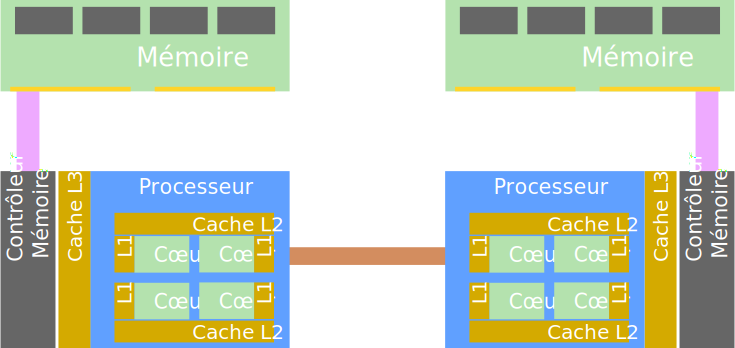
\includegraphics[width=0.8\textwidth]{numa_architecture}
  \caption{Exemple d'une architecture NUMA à deux processeurs.}
  \label{fig:numa_architecture}
\end{figure}

Un autre problème se situe au niveau de la bande passante.
%
La bande passante totale de la machine est distribuée entre chaque banc NUMA.
%
Pour exploiter efficacement la totalité de la bande passante, il faut répartir les données que l'on va utiliser sur tous les bancs mémoires.
%
Des interfaces de programmation existent pour connaître et améliorer la localité des données.
%
Il ne suffit pas de faire une répartition équitable, il faut aussi au moment de l'accès au données que tous les coeurs de calcul accède à des données différentes qui doivent se situer dans la mémoire qui leur est la plus proche.
